\documentclass[10pt,a4paper,sans]{moderncv}

% Temi di ModernCV
\moderncvstyle{banking}
\moderncvcolor{blue}

% Impostazioni pagina e lingua
\usepackage[utf8]{inputenc}
\usepackage[T1]{fontenc}
\usepackage{lmodern}
\usepackage[italian]{babel}
\usepackage[scale=0.88]{geometry}

% Librerie grafiche avanzate
\usepackage{fontawesome5}
\usepackage[most]{tcolorbox}
\usepackage{tikz} % Per il posizionamento della foto
\tcbuselibrary{breakable}

% --- DEFINIZIONI GRAFICHE ---
\newtcolorbox{socialbox}{
  colback=blue!5!white,
  colframe=blue!75!black,
  fonttitle=\bfseries,
  title=Esperienza Sociale \& Soft Skills,
  enhanced,
  breakable,
  before skip=3mm,
  after skip=3mm,
  attach boxed title to top left={xshift=2mm,yshift=-2mm},
  boxed title style={colback=blue!75!black}
}

\newcommand{\cvbadge}[1]{%
  \tcbox[on line, boxsep=0pt, left=4pt, right=4pt, top=2pt, bottom=2pt, colback=gray!20, colframe=gray!20, boxrule=0pt, fontupper=\sffamily\scriptsize\bfseries, arc=2pt]{#1}%
}

% --- DATI PERSONALI ---
\name{Antonio}{Scharmuller}
\title{Studente di Informatica | Aspirante Backend Developer}
\address{Medicina (BO)}{Italy}{}
\phone[mobile]{+39~339~4823393}
\email{scharmullerantonio@gmail.com}
\social[linkedin]{tuo-profilo-linkedin}
\social[github]{Swarz04}

\begin{document}

% INIZIO STRUTTURA A DUE COLONNE
\begin{minipage}[t]{0.70\textwidth}
\vspace{0pt} % Forza l'allineamento in alto assoluto

% --- INTESTAZIONE MANUALE ---
{\fontsize{24}{28}\selectfont\textcolor{color1}{Antonio \textbf{Scharmuller}}}\\[1ex]
{\large\textcolor{darkgray}{Studente di Informatica | Aspirante Backend Developer}}\\[1ex]
{\color{color1}\rule{\textwidth}{0.4pt}}\vspace{3mm}

\section{Profilo Professionale}
Studente di Informatica presso l'Università di Bologna focalizzato sullo sviluppo \textbf{Backend}. Unisco solide basi tecniche (Java, Python, SQL) a una spiccata capacità di gestione dello stress eproblem solving, maturata in contesti ad alta responsabilità.

\section{Esperienze Lavorative e nel Sociale}



\vspace{2mm}

{\noindent\textbf{Tutor di Informatica e Matematica} \hfill \textit{2023--In corso}\newline
\textit{Centro Estivo Comunale e Privatamente}, Medicina (BO)}\\[1mm]
{\small
Attività costante di supporto allo studio e mentoring per numerosi ragazzi delle scuole medie e superiori, sia in contesti comunali che privati:
\vspace{1mm}
\begin{itemize}
  \item \textbf{Mentoring Tecnico:} Supporto nell'apprendimento di Informatica e Matematica, con particolare focus sulla semplificazione di concetti complessi (logica, algoritmi, basi matematiche).
  \item \textbf{Responsabilità e Supervisione:} Presso il Centro Estivo "L'isola che non c'è", gestione dei gruppi, supervisione delle attività e controllo del rispetto delle regole.
  \item \textbf{Capacità Espositiva:} Sviluppo di doti di pazienza e chiarezza nella spiegazione, competenze fondamentali per un developer che deve collaborare con colleghi e stakeholder.
\end{itemize}
}

\begin{socialbox}
  \textbf{Tirocinante poi Operatore (Area Disabilità) 08/2023-08/2023 08/2024-08/2024 12/2024-12/2024 08/2025-08/2025  } \hfill \textbf{2023 -- 2025} \\
  \textit{Supporto e assistenza a persone con disabilità grave e gravissima.}\\[1ex]
  Questa esperienza quadriennale ha consolidato competenze fondamentali per il profilo professionale:
  \begin{itemize}
    \item \textbf{Affidabilità:} Assunzione di responsabilità dirette sulla sicurezza e il benessere di soggetti fragili.
    \item \textbf{Comunicazione:} Capacità di mediazione e ascolto attivo, essenziali per il lavoro in team.
  \end{itemize}

\end{socialbox}

\section{Progetti Software dal 2025}
\cvitem{S.A.G.E.}{\textbf{Sistema Gestione Spese} \cvbadge{\faDatabase\ SQL} \cvbadge{\faJava\ Java} \newline Sviluppo di un sistema per il monitoraggio finanziario personale con analisi dei dati.}
\vspace{1mm}
\cvitem{UniTiles}{\textbf{Personal Project} \cvbadge{\faJava\ Java} \newline Progetto software personale focalizzato sulla gestione dei materiali universitari e no solo, tramite un'interfaccia intuitiva che facilita l'accesso alle informazioni (siti,virtuali,comandi esguibili in cmd,) e un sistema di note con calendario.}
\vspace{1mm}
\cvitem{MakeAnIceCream}{\textbf{Progetto OOP25} \cvbadge{\faCogs\ OOP} \cvbadge{\faLayerGroup\ Design Patterns} \newline Progetto accademico mirato all'applicazione avanzata dei principi della programmazione ad oggetti.}
\vspace{1mm}
\cvitem{\faGithub\ Altro}{\textit{Codice sorgente e numerosi altri progetti sono consultabili sul mio account GitHub.}}

\section{Istruzione e Formazione}
{\noindent\textbf{Laurea Ingegneria delle Scienze Informatiche} \hfill \textit{2024 -- In corso, II° Anno}\newline
\textit{Università di Bologna, campus di Cesena}}\\[1mm]
{\small Corsi focus: algoritmi e strutture dati, Basi di Dati, Programmazione ad Oggetti, Metodi Numerici per l'IA.}

\vspace{2mm}

{\noindent\textbf{Diplomato - Indirizzo Scienze Applicate} \hfill \textit\newline
\textit{Giordano Bruno}, Medicina (BO)}

\section{Interessi per Tesi}
\cvitem{Focus}{Architetture backend per Industrial IoT o Computer Vision applicata al controllo qualità.}

\end{minipage}%
\hfill%
\vrule width 0.4pt% Linea verticale di separazione
\hfill%
\begin{minipage}[t]{0.25\textwidth}
\vspace{0pt} % Forza l'allineamento in alto assoluto con l'altra colonna

% --- FOTO INSERITA NELLA COLONNA ---
{\centering 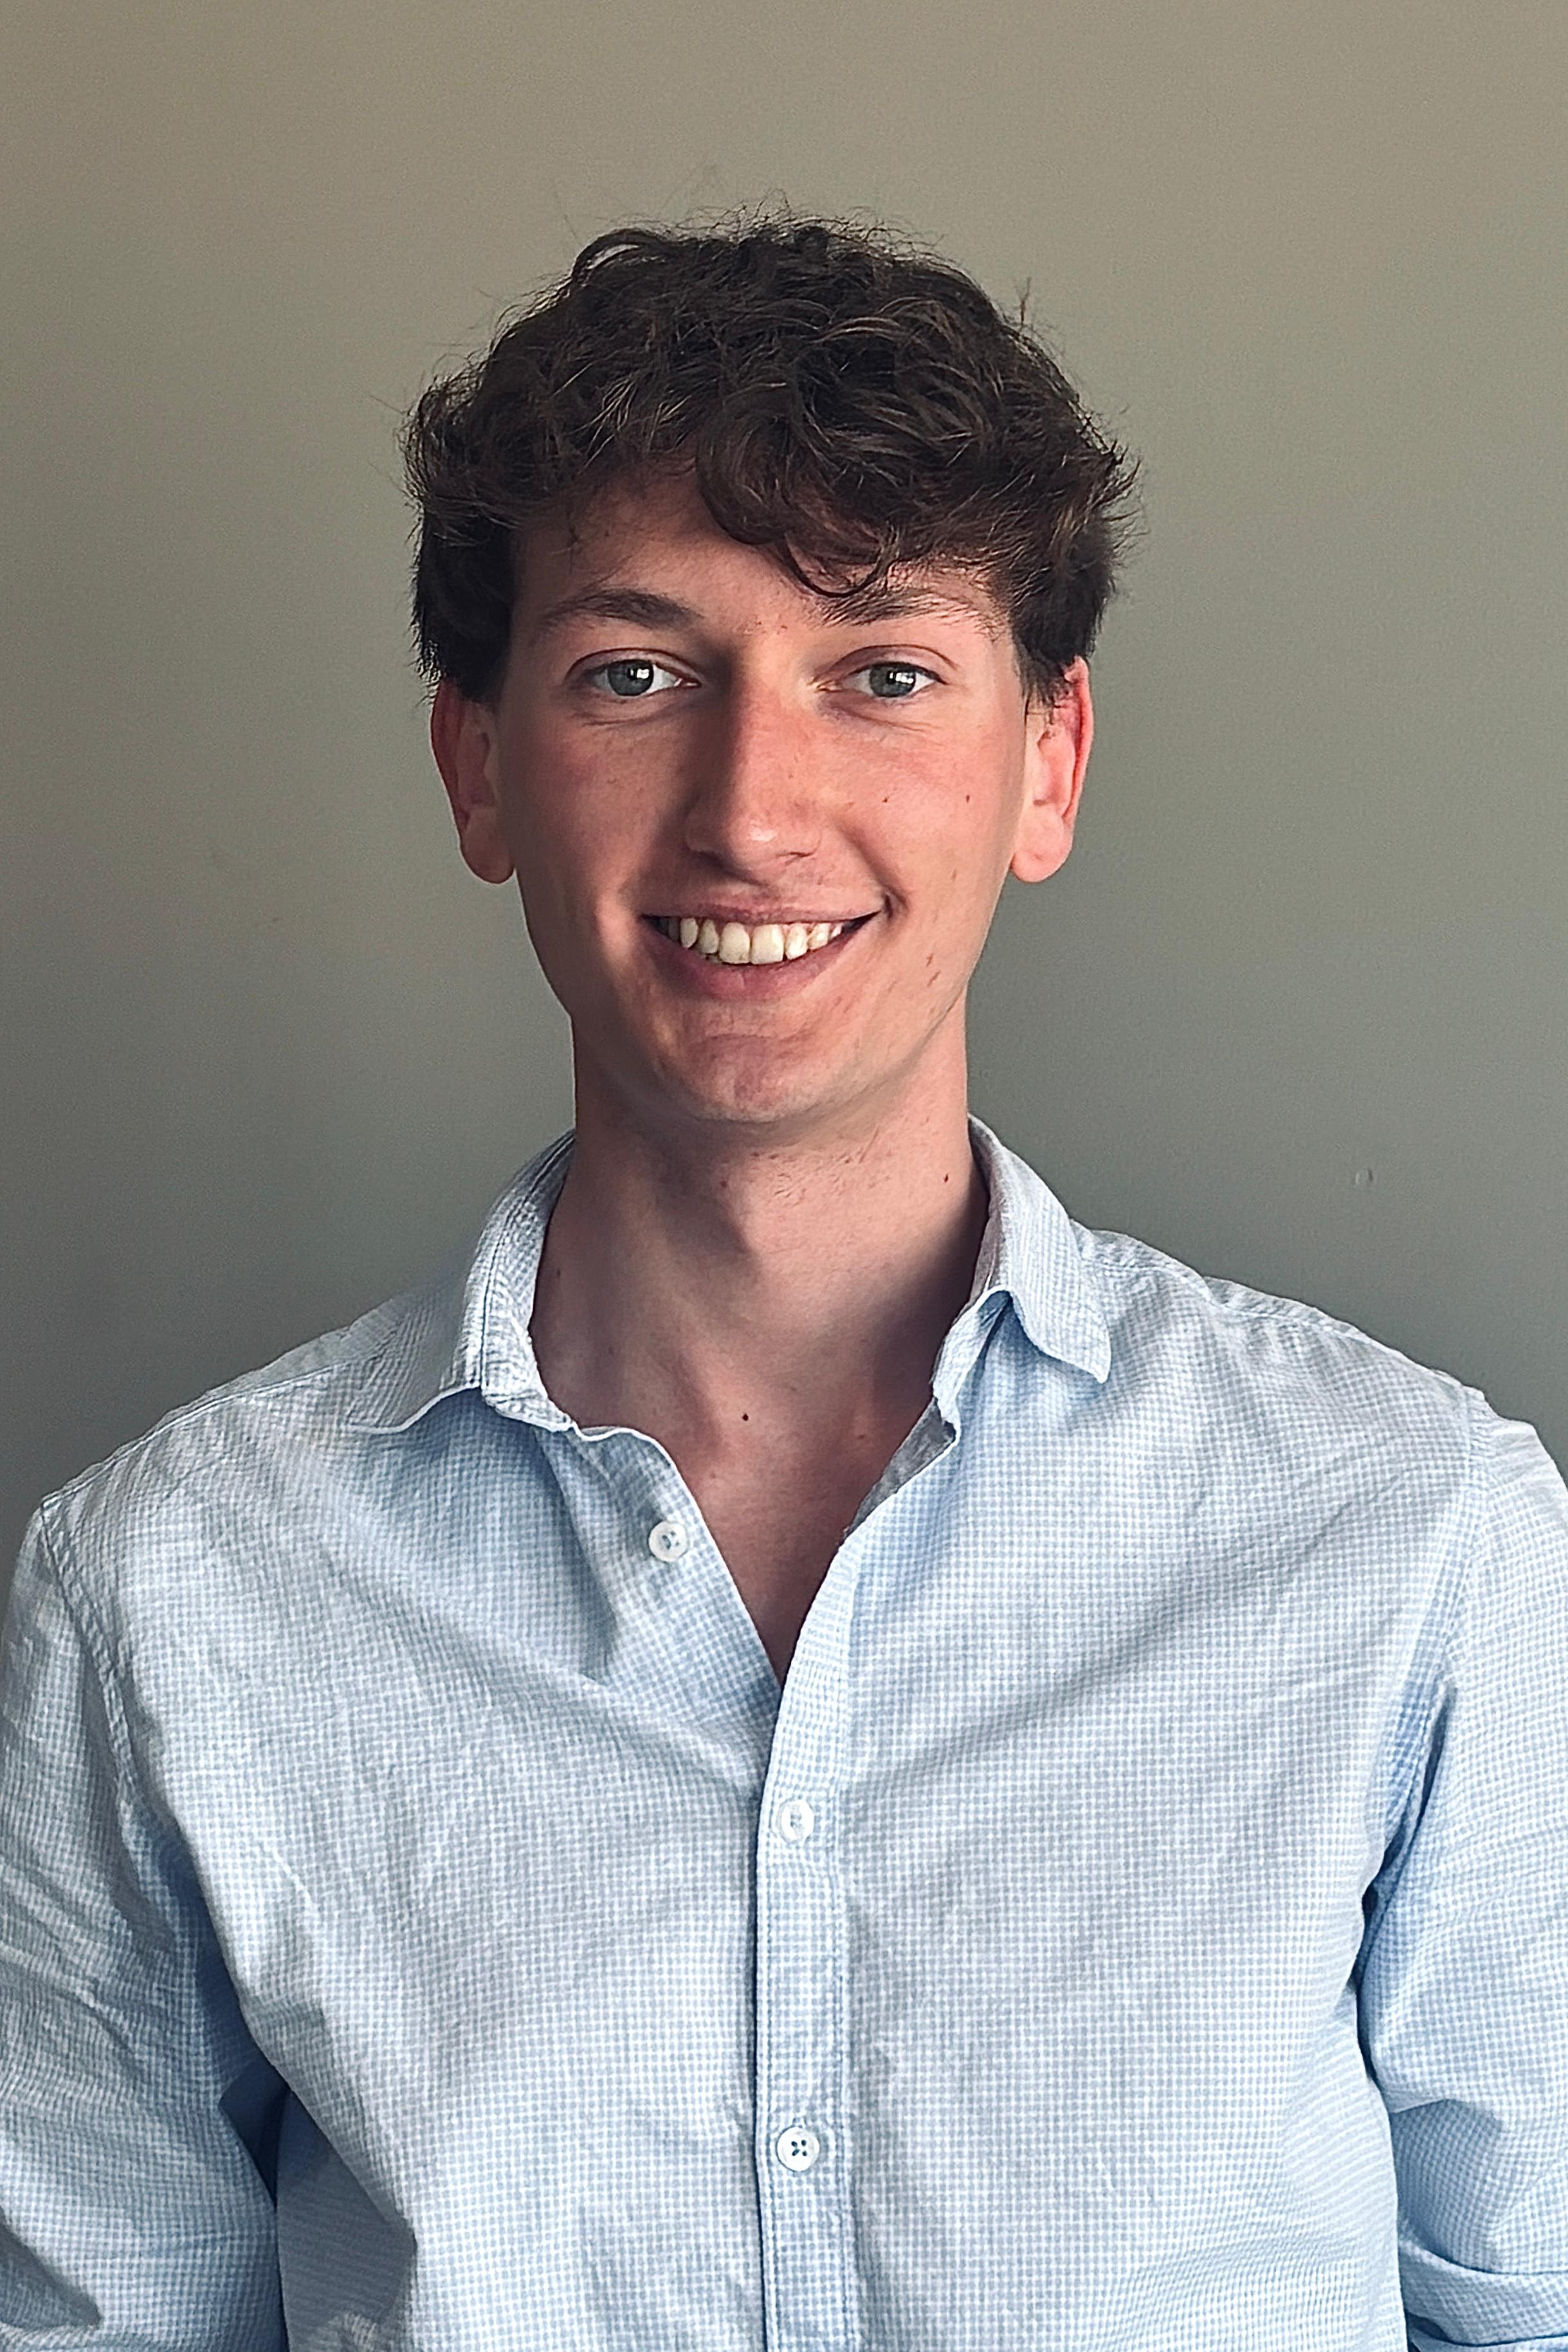
\includegraphics[width=\textwidth, height=6cm, keepaspectratio]{foto.jpeg}\par}

\vspace{2mm}

\section{Contatti Rapidi}
{\small
\faMapMarker\ Medicina (BO) \\[1.5mm]
\faPhone\ +39 339 4823393 \\[1.5mm]
\faEnvelope\ \href{mailto:scharmullerantonio@gmail.com}{scharmullerantonio@gmail.com} \\[1.5mm]
\faLinkedin\ \href{https://linkedin.com/in/tuo-profilo-linkedin}{LinkedIn} \\[1.5mm]
\faGithub\ \href{https://github.com/Swarz04}{Swarz04}
}

\section{Soft Skills}
\vspace{1mm}
\begin{tabular}{@{}l@{\hspace{2mm}}l@{}}
\cvbadge{Problem Solving} & \cvbadge{Professionalità} \\[1.5mm]
\cvbadge{Gestione Stress} & \cvbadge{Affidabilità} \\[1.5mm]
\cvbadge{Team Work} & \cvbadge{Clear Communication} \\[1.5mm]
\cvbadge{Conflict Resolution} & \cvbadge{Time Management} \\[1.5mm]
\end{tabular}

\section{Competenze Tecniche}
\textbf{Linguaggi:}\\
\faJava\ Java, \faPython\ Python\\
\faDatabase\ SQL, C\\[2mm]
\textbf{Sistemi \& Strumenti:}\\
\faServer\ Backend Dev, \faLinux\ Linux\\
\faGit\ Git\\[2mm]
\textbf{Fondamenti:}\\
\faMicrochip\ Architettura, Assembly\\
Arduino, \faHtml5\ HTML, \faCss3\ CSS

\section{Competenze Tecniche}
\textbf{Linguaggi:}\\
\faJava\ Java, \faPython\ Python\\
\faDatabase\ SQL, C\\[2mm]
\textbf{Sistemi \& Strumenti:}\\
\faServer\ Backend Dev, \faLinux\ Linux\\
\faGit\ Git\\[2mm]
\textbf{Fondamenti:}\\
\faMicrochip\ Architettura, Assembly\\
Arduino, \faHtml5\ HTML, \faCss3\ CSS

\end{minipage}
\end{document}
